\documentclass{article}

\usepackage{hcar}
\usepackage{graphicx}
\usepackage{paralist}

\begin{document}

% diagrams-Bd.tex
\begin{hcarentry}[updated]{diagrams}
\report{Brent Yorgey}%11/12
\status{active development}
\participants{Daniel Bergey, Jan Bracker, Andy Gill, Chris Mears, Michael Sloan, Ryan Yates}
\makeheader

The diagrams framework provides an embedded domain-specific language
for declarative drawing.  The overall vision is for diagrams to become
a viable alternative to DSLs like MetaPost or Asymptote, but with the
advantages of being \emph{declarative}---describing what to draw, not
how to draw it---and \emph{embedded}---putting the entire power of
Haskell (and Hackage) at the service of diagram creation.  There is
still much more to be done, but diagrams is already quite
fully-featured, with a comprehensive user manual, a large collection
of primitive shapes and attributes, many different modes of
composition, paths, cubic splines, images, text, arbitrary monoidal
annotations, named subdiagrams, and more.

%**<img width=500 src="./paradox.jpg">
%*ignore
\begin{center}
\includegraphics[width=0.47\textwidth]{html/paradox.jpg}
\end{center}
%*endignore

\subsubsection*{What's new}

Since the last HCAR edition, version 0.6 was released in December.
New features in 0.6 include:
\begin{itemize}
\item A new Haskell-native SVG backend now comes ``out of the
  box''---making installation of diagrams far easier for many users,
  since it no longer depends on any external libraries via the
  FFI. There is also a new official Postscript backend.  The cairo
  backend is still supported, but is no longer required to use
  diagrams.
\item ``Traces'', which give an easy way to find arbitrary points on
  the boundary of a diagram (useful for, \emph{e.g.} drawing
  connecting lines between diagrams).
\end{itemize}

Perhaps the most exciting news since the last HCAR edition is the
release of the \texttt{diagrams-haddock} package, which enables
embedding diagrams code directly in Haddock documentation, with images
automatically compiled and inserted into the Haddock output.  This is
an easy way to spruce up your documentation with declaratively
constructed graphics.  \texttt{diagrams-haddock} is already in use
in a few packages on Hackage, most notably \texttt{diagrams-contrib}.

%**<img width=400 src="./diagrams-haddock.jpg">
%*ignore
\begin{center}
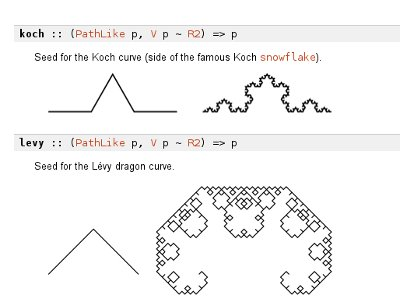
\includegraphics[width=0.4\textwidth]{html/diagrams-haddock.jpg}
\end{center}
%*endignore

In conjunction with \texttt{diagrams-haddock}, there have also been
significant improvements to the underlying \texttt{diagrams-builder}
package, which renders diagrams dynamically at run time.  The caching
and conditional rebuilding of diagrams is now much smarter, so that it
``does the right thing'' in most situations (rebuilding a diagram when
it has changed, and avoiding a rebuild it when it hasn't).  This
directly improves the experience of using \texttt{diagrams-haddock} as
well as \texttt{BlogLiterately-diagrams} (for writing blog posts with
embedded diagrams) and \texttt{diagrams-latex} (for \LaTeX\ documents
with embedded diagrams).

There have been many improvements and changes to the core
diagrams libraries as well, with an 0.7 release planned for the
not-too-distant future. Features slated for the upcoming release
include:
\begin{itemize}
\item A nice API for drawing arrows between arbitrary points or diagrams.
\item Additions to the \texttt{diagrams-contrib} library, including a
  symmetric layout algorithm for binary trees, circle packing layout, a
  generalized turtle drawing interface, factorization diagrams, and
  iterated subset fractals.
\item Computing the curvature of path segments at a given point.
\item Generating paths as a constant offset from another path.
\item A generalized color API, allowing backends to use whatever color
  space they want.
\item Many documentation improvements, using \texttt{diagrams-haddock}
  to  generate example images.
\end{itemize}

%**<img width=350 src="./PythagoreanTree.png">
%*ignore
\begin{center}
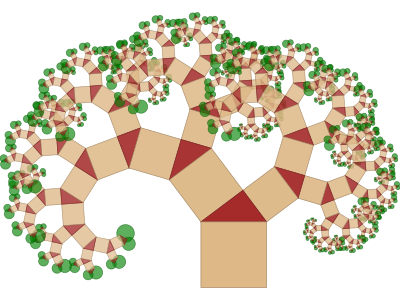
\includegraphics[width=0.235\textwidth]{html/PythagoreanTree.png}
\end{center}
%*endignore


%**<img width=350 src="./FibCalls.png">
%*ignore
\begin{center}
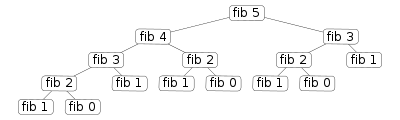
\includegraphics[width=0.33\textwidth]{html/FibCalls.png}
\end{center}
%*endignore

\subsubsection*{Contributing}

There is plenty of exciting work to be done; new contributors are
welcome!  Diagrams has developed an encouraging, responsive, and fun
developer community, and makes for a great opportunity to learn and
hack on some ``real-world'' Haskell code.  Because of its size,
generality, and enthusiastic embrace of advanced type system features,
diagrams can be intimidating to would-be users and contributors;
however, we are actively working on new documentation and resources to
help combat this.  For more information on ways to contribute and how
to get started, see the Contributing page on the diagrams wiki:
\url{http://haskell.org/haskellwiki/Diagrams/Contributing}, or come
hang out in the \texttt{\#diagrams} IRC channel on freenode.

%**<img width=400 src="./tree500.jpg">
%*ignore
\begin{center}
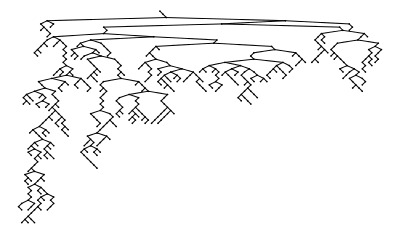
\includegraphics[width=0.4\textwidth]{html/tree500.jpg}
\end{center}
%*endignore

\FurtherReading
\begin{compactitem}
\item \url{http://projects.haskell.org/diagrams}
\item \url{http://projects.haskell.org/diagrams/gallery.html}
\item \url{http://haskell.org/haskellwiki/Diagrams}
\item \url{http://github.com/diagrams}
\item
  \url{https://byorgey.wordpress.com/2012/08/28/creating-documents-with-embedded-diagrams/}
\item \url{http://www.cis.upenn.edu/~byorgey/pub/monoid-pearl.pdf}
\item \url{http://www.youtube.com/watch?v=X-8NCkD2vOw}
\end{compactitem}
\end{hcarentry}

\end{document}